\section{The POP Process}
\label{sec:popp}

The partially observable Poisson process (POPP) is a counting process $N(t)$ with arrival rate $\lambda$ where the number of events that occurred up to time $t$ are obtained by unreliable (possibly multiple) counters. The definition brings a distinction between \emph{true count} (or simply \emph{count}), which refers to the number of events that actually happened, and the \emph{sensed count}, which refers to the count obtained by a counter (or sensor). Given that $c_i$ number of events happened (as the true count) over the interval $[0, t)$ during the $i$-th observation, and $m$ counters observed the events unreliably, thus the sensed count $s_{ji}$ is the count given by sensor $j$ in the $i$-th observation within the interval $[0, t)$ with $0 \leq j \leq m$. 

\begin{figure}[t!]
	\centering
	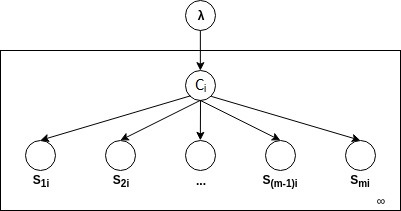
\includegraphics[width=0.5\textwidth]{./figures/gm_popp.jpg}
    \caption{Graphical representation of the partially observable Poisson process.}
	\label{fig:gm_popp}
\end{figure}

The graphical model, which is easily derived from the definition of the POPP, shows that the true count $c_i$ has become a latent variable which can only be inferred from the sensed count $\overrightarrow{s_i} = (s_{1i}, \ldots, s_{mi})$ where each $s_{ji}$ is a sensed count coming from sensor $j$. The posterior of $\lambda$ is then inferred from the posterior of $c_i$ after multiple samples $i = 1 \ldots n$.

A statistical inference to estimate the rate parameter $\lambda$ of the POPP model is done with a marginalisation over all possible true count value $c_i$ in a joint distribution between the posterior $P(\lambda ; c_i)$ and the posterior over $c_i$ given $\overrightarrow{s_i}$. The posterior of $\lambda$, given $n$ samples $\overrightarrow{s}=(\overrightarrow{s_1} \dots \overrightarrow{s_n})$, each consisting of $m$ sensors, is:
\begin{equation}
	\label{eq:marginal_occurrences}
	\begin{tabular}{r@{=}l}
		$P(\lambda ; \overrightarrow{s})$ &  $\displaystyle\sum_{c_1=0}^{\infty} \ldots \displaystyle\sum_{c_n=0}^{\infty} P(\lambda ; \overrightarrow{c}) ~ P(\overrightarrow{c} ; \overrightarrow{s})$ \\
	\end{tabular}
\end{equation}
\noindent where
\begin{equation*}
	\begin{tabular}{r@{ = }l}
		$P(\lambda ; \overrightarrow{c})$ & $Gam\Bigg(\lambda ; \displaystyle\sum_{i=1}^{n} c_i + \alpha, n + \beta \Bigg)$
	\end{tabular}
\end{equation*}
\noindent with $\overrightarrow{c} = (c_1, \ldots, c_n)$ for $1 \leq i \leq n$.

$P(\overrightarrow{c} ; \overrightarrow{s})$ is factored based on the assumption that each sensor is \textit{uncorrelated} to one another given the true count $c_i$. Consequently, the probability that the vector of true counts is $\overrightarrow{c}$, given $n$ samples of the vector of $m$ sensed counts $\overrightarrow{s_1}, \ldots, \overrightarrow{s_n}$, is

\begin{equation}
    \label{eq:occurrences_likelihood}
    \begin{tabular}{r@{ $\varpropto$ }l}
        $P(\overrightarrow{c} ; \overrightarrow{s_1}, \ldots, \overrightarrow{s_n})$ & $P(\overrightarrow{s_1}, \ldots, \overrightarrow{s_n} ; \overrightarrow{c}) ~ P(\overrightarrow{c})$ \\ [1ex]
        & $\displaystyle\prod_{i=1}^{n} P(\overrightarrow{s_i} ; c_i) ~ P(c_i)$ \\ [2ex]
        & $\displaystyle\prod_{i=1}^{n} \displaystyle\prod_{j=1}^{m} P(s_{ji} ; c_i) ~ P(c_i ; \overrightarrow{c_{-1}})$
    \end{tabular}
\end{equation}

\noindent where $\overrightarrow{c_{-1}} = c_{i-1}, \ldots, c_1$.

$P(c_i ; \overrightarrow{c_{-1}})$ and $P(s_{ji} ; c_i)$ are defined to complete Eqn. \ref{eq:occurrences_likelihood}. $P(c_i ; \overrightarrow{c_{-1}})$ is calculated in the form of a negative binomial distribution

\begin{equation}
	\label{eq:unconditional_xi}
	\begin{tabular}{r@{=}l}
		$P(c_i ; \overrightarrow{c_{-1}})$ & $\displaystyle\int_{\lambda=0}^{\infty} P(c_i ; \lambda) ~ P(\lambda ; \overrightarrow{c_{-1}}) ~d\lambda$ \\ [2ex]
		& $\displaystyle\int_{\lambda=0}^{\infty} Poi(c_i ; \lambda) ~ Gam(\lambda ; \alpha, \beta) ~d\lambda$ \\ [2ex]
		& $NB\Bigg(c_i ; \alpha, \displaystyle\frac{\beta}{\beta + 1}\Bigg)$.
	\end{tabular}
\end{equation}

The Poisson limit theorem states that the Poisson distribution may be used as an approximation to the binomial distribution \cite{papoulis2002probability}. Using this theorem as the foundation, an arbitrarily close approximation to the probability $P(s_{ji} ; c_i)$ is defined by assuming there exists a small enough finite subinterval of length $\delta$ for which the probability of more than one event occurring is less than some small value $ \epsilon$. With this assumption, interval $[0, t)$ is splitted into $l$ smaller subintervals $I_1, \ldots, I_l$ of equal size, with the condition that $l > \lambda$ (the condition is crucial since we focus on very small portions of the interval). Consequently, the whole interval $[0, t) = I_1, \ldots, I_l$ becomes a series of Bernoulli trials, where the $k^{th}$ trial corresponds to whether (1) an event $e_k$ happens with probability $\lambda / l$ and (2) a sensor $j$ captures the event $e_k$ as the detection $d_k$ at the subinterval $I_k$.

$P(s_{ji} ; c_i)$ is defined as the aggregate of the true positives $tp_{ji}$ in $c_i$ subintervals, and the false positives $fp_{ji}$ in $l-c_i$ subintervals. The probability of a \textit{true positive detection} (TP) for sensor $j$ in a subinterval is $tpr_j = P_j(d = 1 ; e=1)$, and the probability of a \textit{false positive detection} (FP) is $fpr_j = P_j(d = 1 ; e=0)$. Thus $P(s_{ji} ; c_i)$ is defined as a sum of two binomial distributions $B(r ; n,\pi)$, where the aggregate is constrained to be $s_{ji}$: 

\begin{equation}
	\label{eq:joint_binomial_distribution}
    P(s_{ji} ; c_i) \! = \! \! \! \displaystyle\sum_{\textrm{tp}_{ji} = 0}^{c_{i}} \! \! B\Big(\textrm{tp}_{ji} ; c_i, \textrm{tpr}_j\Big) B\Big(\textrm{fp}_{ji} ; \Delta c_i, \textrm{fpr}_j \Big)
\end{equation}
\noindent where $s_{ji} = \textrm{tp}_{ji} + \textrm{fp}_{ji}$, $\textrm{tpr}_j = P_j(d=1 ; e=1)$, $\textrm{fpr}_j = P_j(d=1 ; e=0)$, and $\Delta c_i = (l - c_i)$.

Eqn.~\ref{eq:marginal_occurrences} shows the difficulty of belief state estimation in the POPP model since there is no conjugate density accomodating an analytical solution for the posterior over $\lambda$. Each sensed count sample $\overrightarrow{s_i}$ used to update the posterior of $\lambda$ adds a factor of countably infinite number of elements. The resulting posterior is a sum of countably infinite sums. One can place an upper bound $l$ on the maximum value of each $c_i$, but it still makes the number of elements in the posterior grow by a factor $l$ with every sensed count $\overrightarrow{s_i}$.  

With this difficulty noted, Jovan et al., proposed three efficient estimators, each of which offers an approximation to the true posterior $P(\lambda ; \overrightarrow{s})$. A more detailed presentation of these estimators is given in \cite{jovan18a}.
